\section{Unterschiedliche Charakter}
Spiele verwenden die unterschiedlichsten Charaktere, nicht nur in Bezug auf das Aussehen, sondern auch hinsichtlich der Komplexität der Körperteile und der Anzahl der Knochen. Um den Charaktercontroller vielseitig einsetzbar zu gestalten, werden in diesem Kapitel die Walker-Demo-Komponenten angepasst, um den Einrichtungsprozess zu vereinfachen und unterschiedliche Charakterkörperstrukturen zu ermöglichen. Zunächst wird analysiert, wie das Agentenskript angepasst werden muss, um Charaktere mit unterschiedlichen Körperstrukturen zu steuern und zu trainieren. Anschließend wird der Einrichtungsprozess am Beispiel eines Mixamo-3D-Charaktermodells dargestellt. Zum Schluss wird der Mixamo-Charakter trainiert und das Ergebnis ausgewertet. Die Wahl des Mixamo-Modells als Beispiel soll zeigen, wie die Einrichtung mit den Vereinfachungen funktioniert und wie das Training bei der Verwendung von komplexere Charaktermodelle beeinflusst wird.

\subsection{Anforderungen}	
Der Agent der Walker Demo setzt für jedes Körperteil eine separate Referenz, die über den Inspector in Unity konfiguriert werden muss. Um die damit verbundene Einschränkung einer festgelegten Konfiguration von Körperteilen zu beheben, soll eine flexible Liste von Körperteilen konfiguriert werden. Bei der Zustandserfassung der Körperteile soll anschließend der Zustand aller Körperteile in der Liste erfasst werden. Die Aktion soll gleichermaßen Zielwinkel und Gelenkstärke für alle Körperteile der Liste beinhalten. Um unnötige Komplexität bei der Beobachtung und Aktion zu vermeiden, sollen die Zielwinkel nur für bewegbare Gelenkachsen bestimmt werden. Die Gelenkstärke soll für komplett versteifte Gelenke ebenfalls ausgelassen werden. Um die Konfiguration weiter zu erleichtern, sollen die Körperteile zudem automatisch dem Walker-Agenten hinzugefügt werden. Schließlich soll auch das \hl{Stabilisierungsobjekt} automatisch generiert werden. Diese Änderungen zielen darauf ab, die Flexibilität und Benutzerfreundlichkeit des Walker-Demo-Agenten zu verbessern. Es soll manuelle Konfiguration auf das nötigste reduziert werden, gleichzeitig soll aber auch eine Skalierbare Lösung für unterschiedliche Charakterkörperstrukturen implementiert werden.

\subsection{Anpassungen}
Der Aufbau der Walker-Demo-Skripte, zu sehen in \ref{fig:architektur_alt}, verteilt die Aufgaben auf viele unterschiedliche Komponenten. Diese Aufteilung erschwert die Einrichtung und das Erweitern der Funktionalität erheblich. Die Aufgabenverteilung ist zudem nicht sinnvoll durchdacht. Ein Beispiel dafür ist die Zielsteuerung, die eigenständig funktioniert, während das Stabilisierungsobjekt vom Agenten aktualisiert werden muss.

\begin{figure}[H]
  \centering  
  \begin{tikzpicture}[node distance=3cm]
  
    \node(oc) [rounded] {Stabilisierungsobjekt};  
    \node(agent) [rounded, below of=oc] {Agent};
    \node(target) [rounded, left of=agent, xshift=-2cm] {Zielsteuerung};
    \node(jdc) [rounded, below of=agent] {Motor Gelenk Steuerung};
    \node(bp) [rounded, right of=jdc, xshift=4cm] {Körperteil};
    \node(gc) [rounded, right of=agent, xshift=4cm] {Bodenkontakt};
    
    \draw [uni] (agent) -- (oc) node[midway, right] {aktualisiert Ausrichtung};
    \draw [uni] ([shift={(0.5,-0.5)}] agent.center) -- ([shift={(0.5,0.5)}] jdc.center) node[midway, right, align=center] {initialisierung\\Körperteile};
    \draw [uni] ([shift={(-0.5,0.5)}] jdc.center) -- ([shift={(-0.5,-0.5)}] agent.center) node[midway, left, align=center] {Körperteil-\\liste};
    \draw [uni] (jdc) -- (bp) node[midway, above] {initialisierung};
    \draw[uni] ([shift={(0, 0.3)}] gc.west) -- ([shift={(0, 0.3)}] agent.east) node[midway, above] {frühes stoppen};
    \draw [uni] ([shift={(0, -0.3)}] agent.east) -| ([shift={(-1,0.5)}] bp.center) node[midway, left, yshift=-0.2cm] {steuert};
    \draw[uni] (bp) -- (gc) node[midway, right] {hat};
    \draw [uni] (target) to[loop below] () node [yshift=-1.5cm, align=center] {setzt neue\\Position};
        
  \end{tikzpicture}
  \caption{Alte Architektur}
  \label{fig:architektur_alt}
\end{figure}

Im neuen Ansatz (siehe Abbildung \ref{fig:architektur_neu}) wird die Steuerung und die Datenhaltung der Körperteile in eine Unitykomponente integriert. Zudem wird der Ablauf des Lernprozesses vollständig im Agenten implementiert. Externe Objekte wie die Zielsteuerung oder das Stabilisierungsobjekt werden, wo nötig, vom Agenten erstellt. Das Stabilisierungsobjekt benötigt, sobald es einmal initialisiert ist, keinen weiteren Input für die Aktualisierung der Ausrichtung. Aus diesem Grund wird die Aktualisierung fortan vom Stabiliserungsobjekt selbst ausgeführt. Um mehr Kontrolle über die Zielsetzung zu erlangen, wird die Zielsetzung über ein Event vom Agenten ausgelöst. Die Funktionen der Bodenkontaktkomponente werden zuletzt ebenfalls in die Körperteilkomponente verschoben, um doppelte Konfigurationen von Referenzen zu reduzieren. Als Ergebnis dieser Umstrukturierung kann der Agent als Gehirn des Läufers interpretiert werden, während die Körperteile die Muskeln und Nerven darstellen. Diese neue Architektur bietet den Vorteil, dass die Körperteilkomponenten der Unterobjekte vom Agenten beim Programmstart als Liste abgefragt werden können, wodurch theoretisch jede beliebige Körperstruktur gesteuert werden kann.

\begin{figure}[H]
  \centering  
  \begin{tikzpicture}[node distance=3cm]
  
    \node(oc) [rounded] {Stabilisierungsobjekt};  
    \node(agent) [rounded, below of=oc] {Agent};
    \node(target) [rounded, left of=agent, xshift=-2cm] {Zielsteuerung};
    \node(bp) [rounded, right of=agent, xshift=3cm] {Körperteil};
    
    \draw [uni] (oc) to[loop above] () node[yshift=1.5cm] {aktualisiert Ausrichtung};
    \draw [uni] (agent) -- (oc) node[midway, right] {erstellt};
    \draw [uni] ([shift={(0,0.3)}]  agent.east) -- ([shift={(0,0.3)}] bp.west) node[midway, above] {steuert};
    \draw [dashed,uni] ([shift={(0,-0.3)}] bp.west) -- ([shift={(0,-0.3)}] agent.east) node[midway, below, align=center] {Event\{bodenkontakt\\Zielberührung\}};
    \draw[uni] (agent) to[loop below] () node[yshift=-1.5cm] {frühes stoppen};
    \draw [dashed, uni] (agent) -- (target) node[midway, above, align=center] {Event\{setzt neue\\Position\}};
        
  \end{tikzpicture}
  \caption{Neue Architektur}
  \label{fig:architektur_neu}
\end{figure}

Um die Steuerung von beliebigen Körperstrukturen zu ermöglichen, müssen zudem die Erstellung der Beobachtung sowie das Ausführen der Aktion je nach Körperstruktur dynamisch angepasst werden. Bei der Initialisierung der Körperteile wird geprüft, ob das Körperteil über eine Gelenkkomponente verfügt. Ist das der Fall, werden die Freiheitsgrade dieser Gelenke bestimmt. Die Freiheitsgrade geben anschließend an, welche Felder für das Körperteil in der Beobachtung hinzugefügt und in der Aktion ausgelesen werden müssen. Die Beobachtung wurde bereits im ursprünglichen Walker-Agent-Skript dynamisch für jedes Körperteil in einer Liste erstellt. Die Aktion wurde jedoch bisher statisch für jedes Körperteil ausgelesen. Im neuen Ansatz, wie in Codeausschnitt \ref{lst:aktion_dynamisch} dargestellt, wird die Aktion nun dynamisch ausgewertet, basierend auf den zuvor ermittelten Freiheitsgraden.

\begin{lstlisting}[caption={Agent Aktion in Bewegung umwandeln},captionpos=b,label={lst:aktion_dynamisch}]
public override void OnActionReceived(ActionBuffers actionBuffers)
    {
        var continuousActions = actionBuffers.ContinuousActions;
        int i = -1;

        foreach (Bodypart bp in bodyparts)
        {
            //Körperteil mit steifem oder keinem Gelenk wird ignoriert
            if (bp.dof.sqrMagnitude <= 0) continue;
            float targetRotX = bp.dof.x == 1 ? continuousActions[++i] : 0; // wenn Gelenk um X-Achse beweglich ist wird Wert aus Aktion ausgelesen
            float targetRotY = bp.dof.y == 1 ? continuousActions[++i] : 0; // - Y-Achse - 
            float targetRotZ = bp.dof.z == 1 ? continuousActions[++i] : 0; // - Z-Achse - 
            float jointStrength = continuousActions[++i];
            bp.SetJointTargetRotation(targetRotX, targetRotY, targetRotZ); //Zielrotation setzen
            bp.SetJointStrength(jointStrength); //Gelenkstärke setzen
        }
    }
\end{lstlisting}

\subsection{Einrichtung}
Der ausgewählte Charakter ist der Y Bot-Charakter, welcher in Abbildung \ref{fig:charakter_mixamo} zu sehen ist. Der Y Bot besteht, ausgenommen der Finger, aus 22 Knochen. Um das Training zu beschleunigen, werden für alle Versuche die Finger mit dem Handknochen als ein Körperteil zusammengefasst. Die Entscheidung, das Skelett zu vereinfachen, ist ein gängiger Ansatz, um die Trainingszeit und -komplexität zu verringern. Durch die Zusammenfassung der Finger mit dem Handknochen wird die Anzahl der zu steuernden Gelenke reduziert, was wiederum die Anzahl der Optionen verringert, die der Agent im Verlauf des Trainings ausprobieren muss.

\begin{figure}[H]
  \centering  
  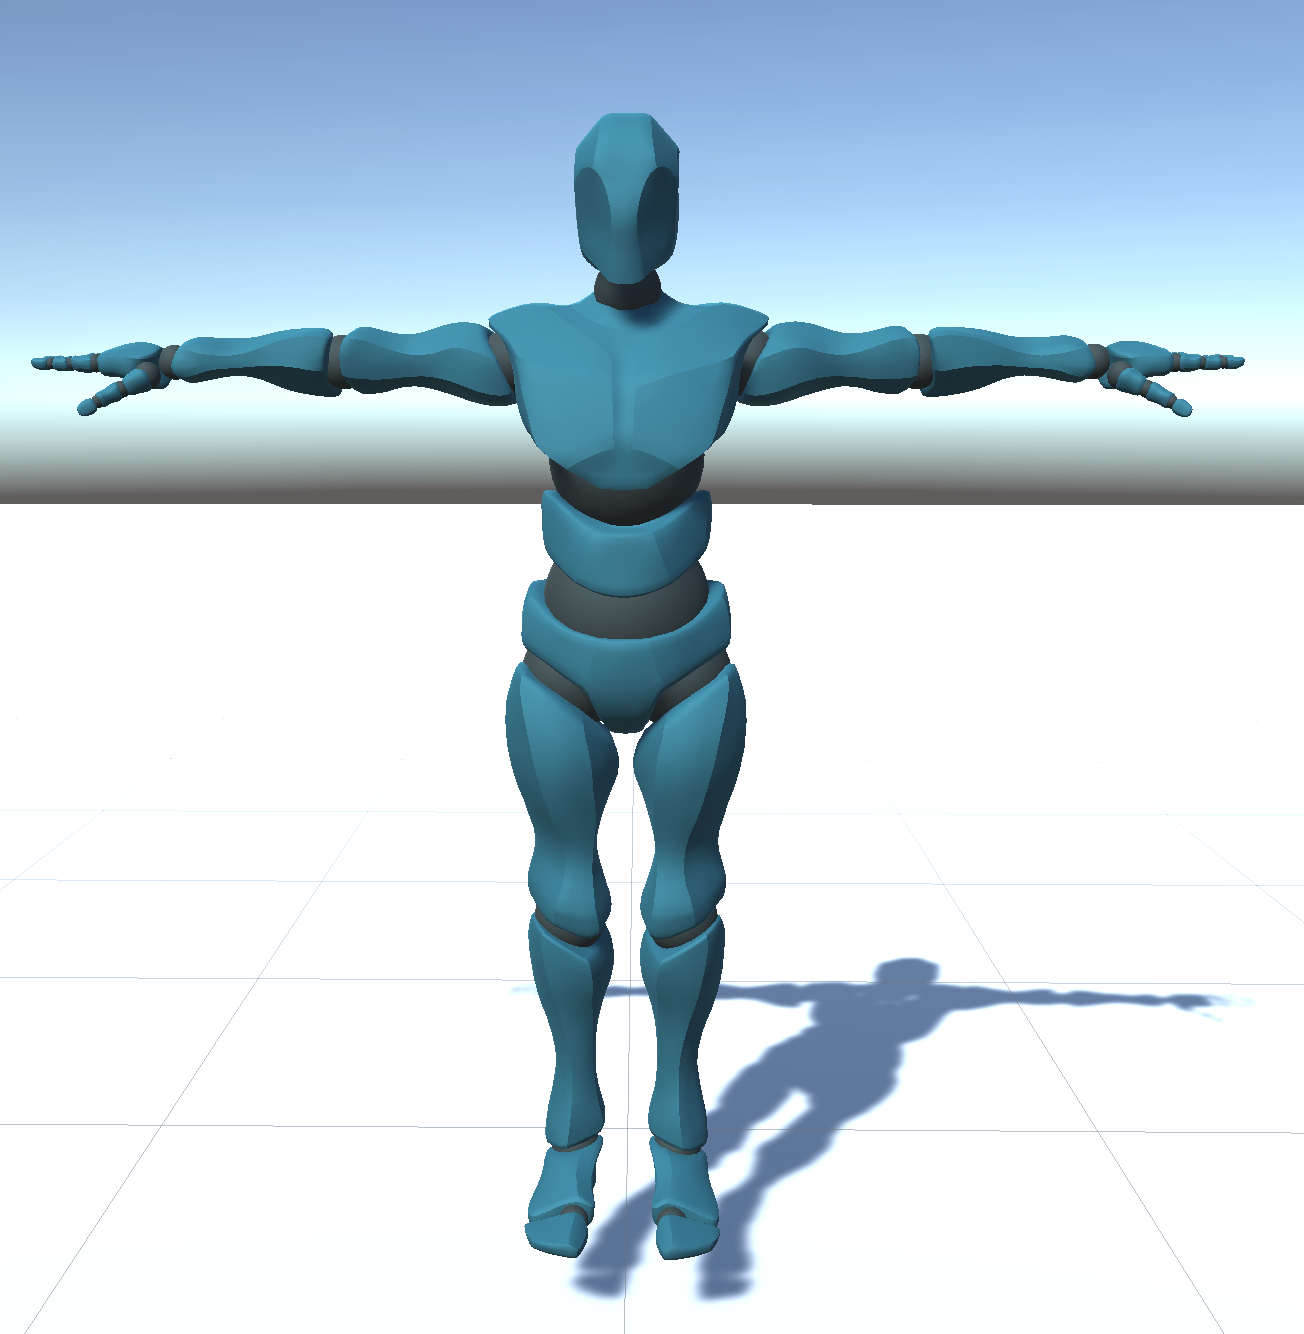
\includegraphics[scale=0.5]{img/charakter_mixamo}
  \caption{Mixamo Charakter Y Bot}
  \label{fig:charakter_mixamo}
\end{figure}

Jedes Körperteil benötigt für das Steuern und Trainieren mit dem Walker Agenten Skript eine Kollisionskomponente, eine Festkörperkomponente und eine Körperteilkomponente. Zusätzlich müssen Gelenkkomponenten hinzugefügt werden, um die Körperteile miteinander zu verbinden. Dabei wird die Gelenkkomponente jeweils auf das untergeordnete Körperteil angewendet, während das übergeordnete Körperteil als verbundener Körper referenziert wird. Die Kollisionskomponente soll das Körperteil in vereinfachter Form und Größe darstellen, um die Berechnungen zu optimieren. Bei den Festkörpern müssen das Gewicht und der Schwerpunkt festgelegt werden, um eine realistische physikalische Simulation zu gewährleisten. In der Gelenkkomponente können Bewegungen durch das Festlegen von Winkellimits gesperrt oder limitiert werden. Für die Rotationsberechnung wird der Slerp-Modus verwendet. Slerp (Spherical Linear Interpolation) ist besonders nützlich in physikbasierten Simulationen, da es eine kontinuierliche und glatte Rotation zwischen zwei Orientierungen gewährleistet, was zu natürlicheren Bewegungen führt. Die Gewichte der Körperteile wurden von der Walker Demo übernommen. Gleichermaßen wurden die Winkellimits für die Gelenke übernommen. Die zusätzlichen Körperteile wurden vereinfacht. Der Oberkörper besteht im Mixamo-Modell aus den Schulterknochen sowie dem obersten Wirbel der Wirbelsäule. Die Wirbelsäule besteht im Mixamo-Modell aus zwei Wirbeln anstatt einem Wirbel des Läufers aus der Demo. Zuletzt sind die Füße noch in Fuß und Vorderfuß aufgeteilt. Bei diesen Änderungen der Körperstruktur wurden die Gewichte und Winkellimits des vereinfachten Körpers auf die komplexeren Körperstrukturen aufgeteilt. Diese Vereinfachungen tragen ebenfalls dazu bei die Komplexität möglichst nah der Walker Demo anzugleichen. In Szenarien mit komplexeren Skills und Bewegungsabläufen kann die Vereinfachung zu Einschränkungen führen. Für das erlernen einer Gehbewegung sind die Vereinfachungen des Oberkörpers jedoch ein kleiner Abstrich für die damit gewonnene Trainingsdauer.

\begin{table}[H]
  \centering
  {\rowcolors{1}{gray!10}{white}
  \begin{tabular}{ |p{3cm}|p{3cm}|p{2cm}|p{4cm}|p{2cm}| }
  \hline
  \textbf{Körpertei}l& \textbf{Verbundenes Körperteil} & \textbf{Gewicht} & \textbf{Winkellimits} & \textbf{Form} \\
  \hline
  Hüfte & - & 15kg & - & Kapsel \\
  \hline
  Wirbel 1 & Hüfte & 6kg & x(-20,20) y(-20,20) z(-15,15) & Kugel \\
  \hline
  Wirbel 2 & Wirbel 1 & 4kg & - & Kugel \\
  \hline
  Wirbel 3 & Wirbel 2 & 3kg & x(-20,20) y(-20,20) z(-15,15) & Kugel \\
  \hline
  Schulter LR & Wirbel 3 & je 2kg& - & Kugel \\
  \hline
  Nacken & Wirbel 3 & 1kg & - & Kugel \\
  \hline
  Kopf & Nacken & 6kg & x(-30,10) y(-20,20) & Kapsel \\
  \hline
  Oberarm LR & Oberkörper & je 4kg & x(-60,120) y(-100,100) & Kapsel \\
  \hline
  Unterarm LR & Oberarm & je 3kg & x(0,160) & Kapsel \\
  \hline
  Hand LR & Unterarm & je 2kg & - & Quader \\
  \hline
  Oberschenkel LR & Hüfte & je 14kg& x(-90,60) y(-40,40) & Kapsel \\
  \hline
  Unterschenkel LR & Oberschenkel & je 7kg &  x(0,120) & Kapsel \\
  \hline
  Fuß LR & Unterschenkel & je 4kg & x(-20,20) y(-20,20) z(-20,20) & Quader \\
  \hline
  Vorderfuß LR & Fuß & je 1kg & - & Quader \\
  \hline
  \end{tabular}}
  \caption{Mixamo Charakter Körperteile}
  \label{table:mixamo_körperteile}
\end{table}

Die Körperteilkomponente übernimmt die Konfigurationsparameter der Gelenkmotorsteuerung (siehe Abbildung \ref{fig:komponente_bodypart}). Parameter wie Stärke und maximale Rotationsgeschwindigkeit können angepasst werden. Die Standardwerte der Walker Demo bieten hier eine solide Grundlage für die meisten Anwendungsfälle. Bei Bedarf kann auch das Feld \grqq{}Trigger Touching Ground\grqq{} aktiviert werden, um ein Event auszulösen, sobald das Körperteil den Boden berührt. Dieses Feature wird verwendet um im Agenten ein frühes Stop auszulösen sobald ein Körperteil den Boden berührt.

\begin{figure}[H]
  \centering  
  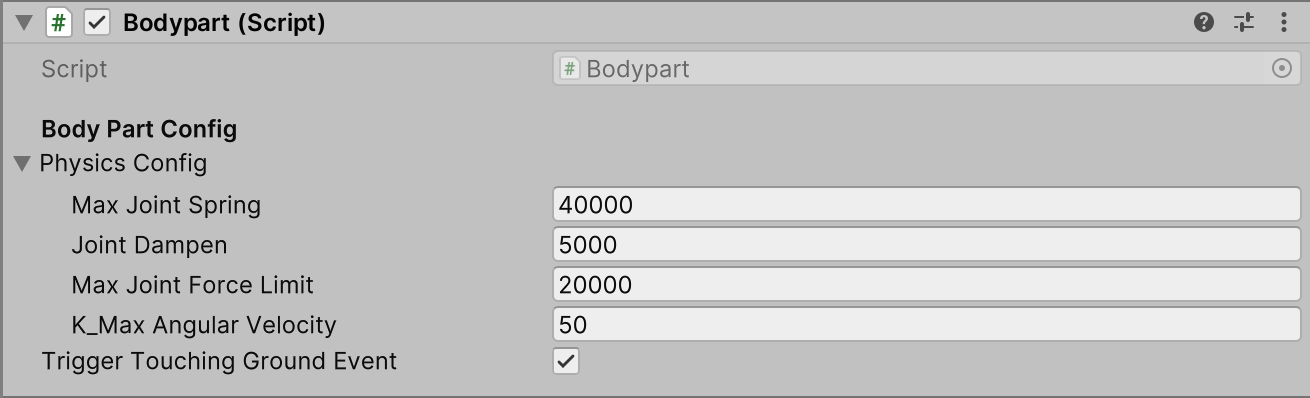
\includegraphics[scale=0.5]{img/komponente_bodypart}
  \caption{Körperteilkomponente}
  \label{fig:komponente_bodypart}
\end{figure}

Ist der Körper fertig konfiguriert, wird zuletzt das Walker Agent Skript zusammen mit den Behaviour-Parametern und dem Decision Requester hinzugefügt. Um die angepasste Walker Agent Komponente nutzen zu können, müssen noch die Referenzen für das Zielobjekt sowie das Hauptkörperteil und den Kopf gesetzt werden. Diese Referenzen werden für die Berechnung von relativen Positionen sowie die Belohnung genutzt. Soll das Ziel bei Berührung neu gesetzt werden, muss auch das Event \grqq{}On Touched Target\grqq{} mit der Platzierungsfunktion der Zielsteuerung verknüpft werden. Zusätzlich können Parameter für das Training, wie Zielgeschwindigkeit und die Zufallsgenerierung der Startrotation, angepasst werden.

\begin{figure}[H]
  \centering  
  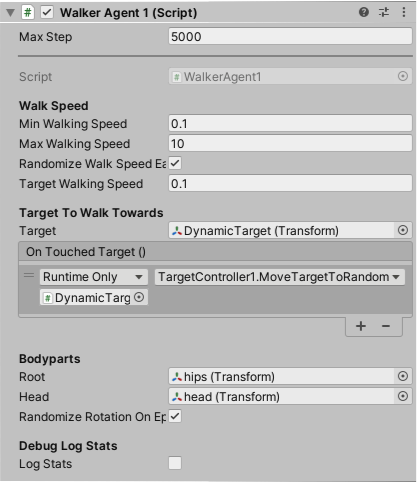
\includegraphics[scale=0.5]{img/komponente_agent_walker1}
  \caption{Walker Agentkomponente}
  \label{fig:komponente_agent_walker1}
\end{figure}

\subsection{Auswertung}
Das Training dauert etwa doppelt so lange, um ein etwas schlechteres Resultat zu erreichen. Der Agent lernt mit dem Mixamo Modell, lange in der Umgebung zu bestehen, und erreicht dabei auch ein gutes Maß an Belohnung pro Schritt (siehe Abbildung \ref{fig:training_mixamo_charakter}). In der Abbildung \ref{fig:mixamo_versuch10_gangbild} wird das erlernte Gangbild gezeigt. Der Läufer lernt in diesem Fall nicht das Laufen, sondern galoppiert zum Ziel. \hl{weiter ausführen???}

\begin{figure}[H]
  \centering  
    \begin{subfigure}{.49\textwidth}
      \centering  
      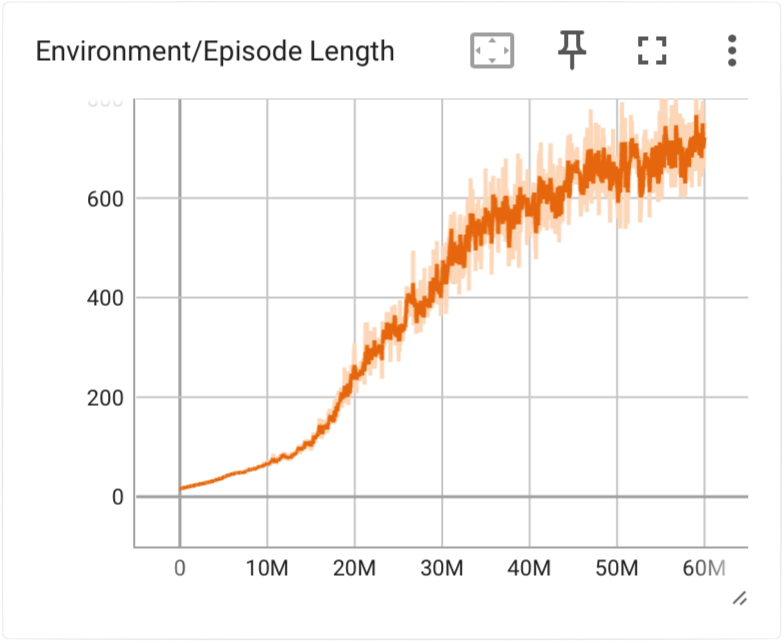
\includegraphics[width=\textwidth]{img/106_episode_length}
      \caption{Episodenlänge}
      \label{fig:106_episode_length}
    \end{subfigure}
    \begin{subfigure}{.49\textwidth}
      \centering  
      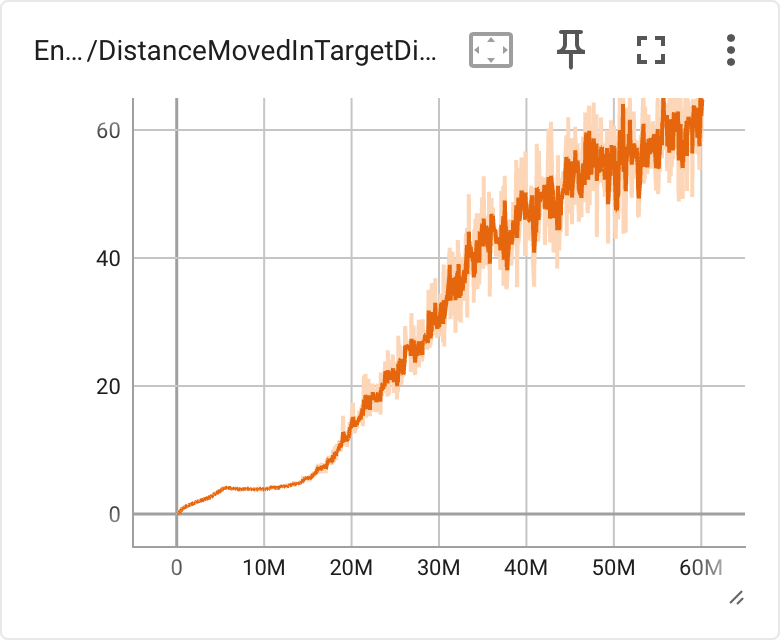
\includegraphics[width=\textwidth]{img/106_move_target_dir}
      \caption{Zurückgelegte Stecke in Zielrichtung}
      \label{fig:106_move_target_dir}
    \end{subfigure}
    \begin{subfigure}{.49\textwidth}
      \centering  
      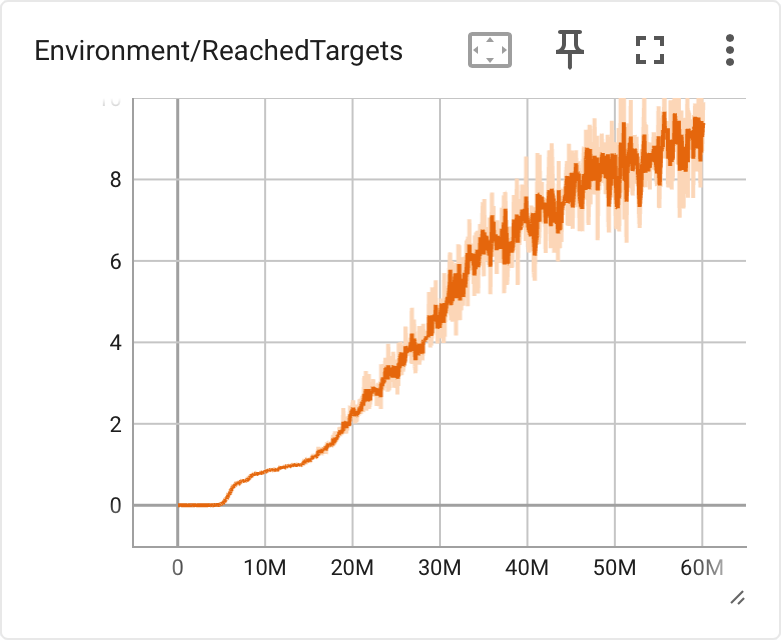
\includegraphics[width=\textwidth]{img/106_reach_target}
      \caption{Erreichte Anzahl an Zielen}
      \label{fig:106_reach_target}
    \end{subfigure}
    \begin{subfigure}{.49\textwidth}
      \centering  
      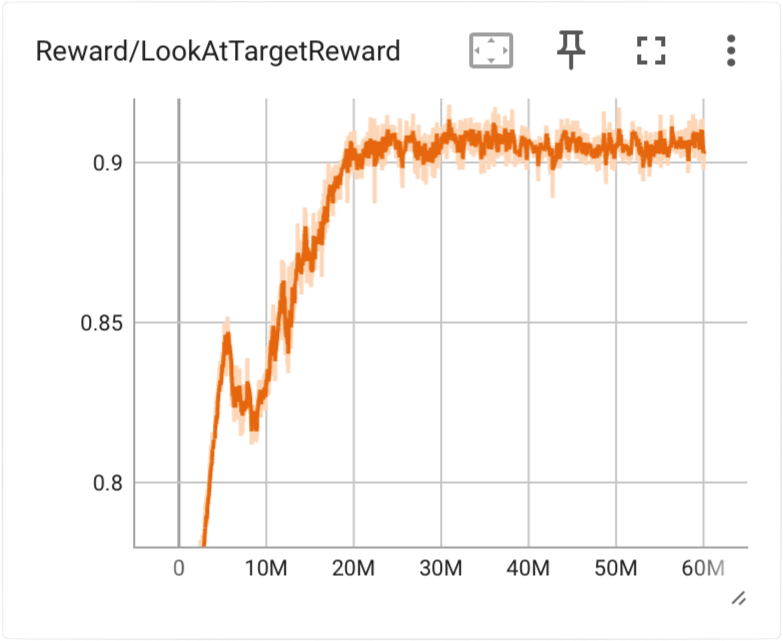
\includegraphics[width=\textwidth]{img/106_look_reward}
      \caption{Blickbelohnung}
      \label{fig:106_look_reward}
    \end{subfigure}
    \begin{subfigure}{.49\textwidth}
      \centering  
      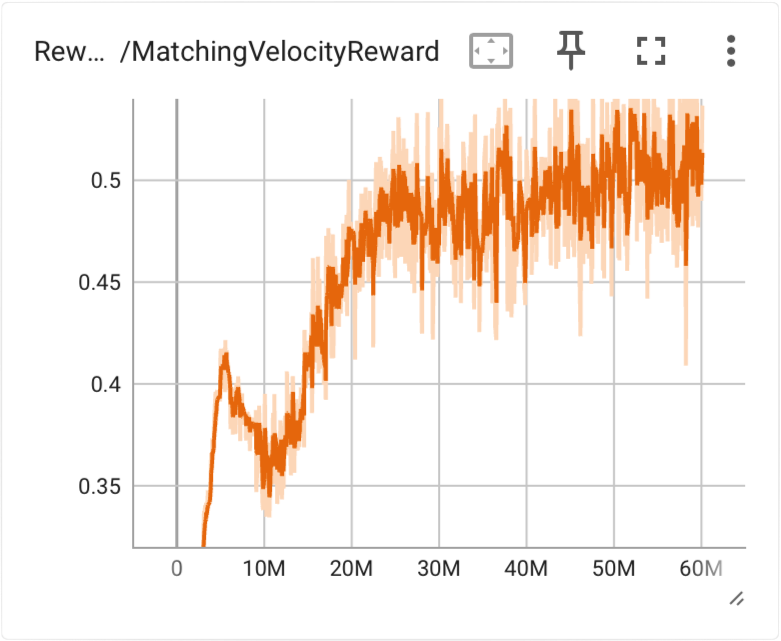
\includegraphics[width=\textwidth]{img/106_vel_reward}
      \caption{Geschwindigkeitsbelohnung}
      \label{fig:106_vel_reward}
    \end{subfigure}
 \caption{Training Mixamo Charakter}
  \label{fig:training_mixamo_charakter}
\end{figure}

\begin{figure}[H]
  \centering
  \begin{tabular}{cccc}
    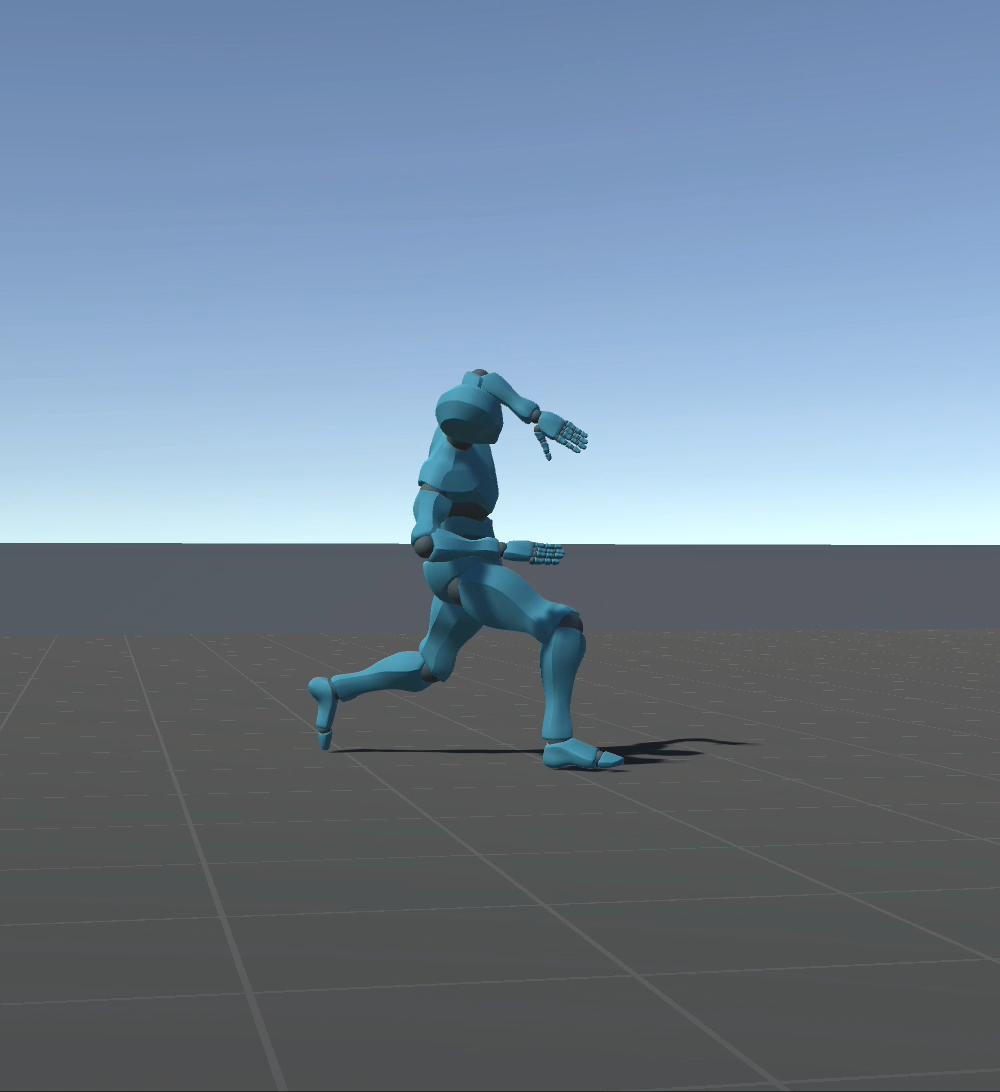
\includegraphics[width=0.2\textwidth]{img/charakter_mixamo_galoppieren1} & 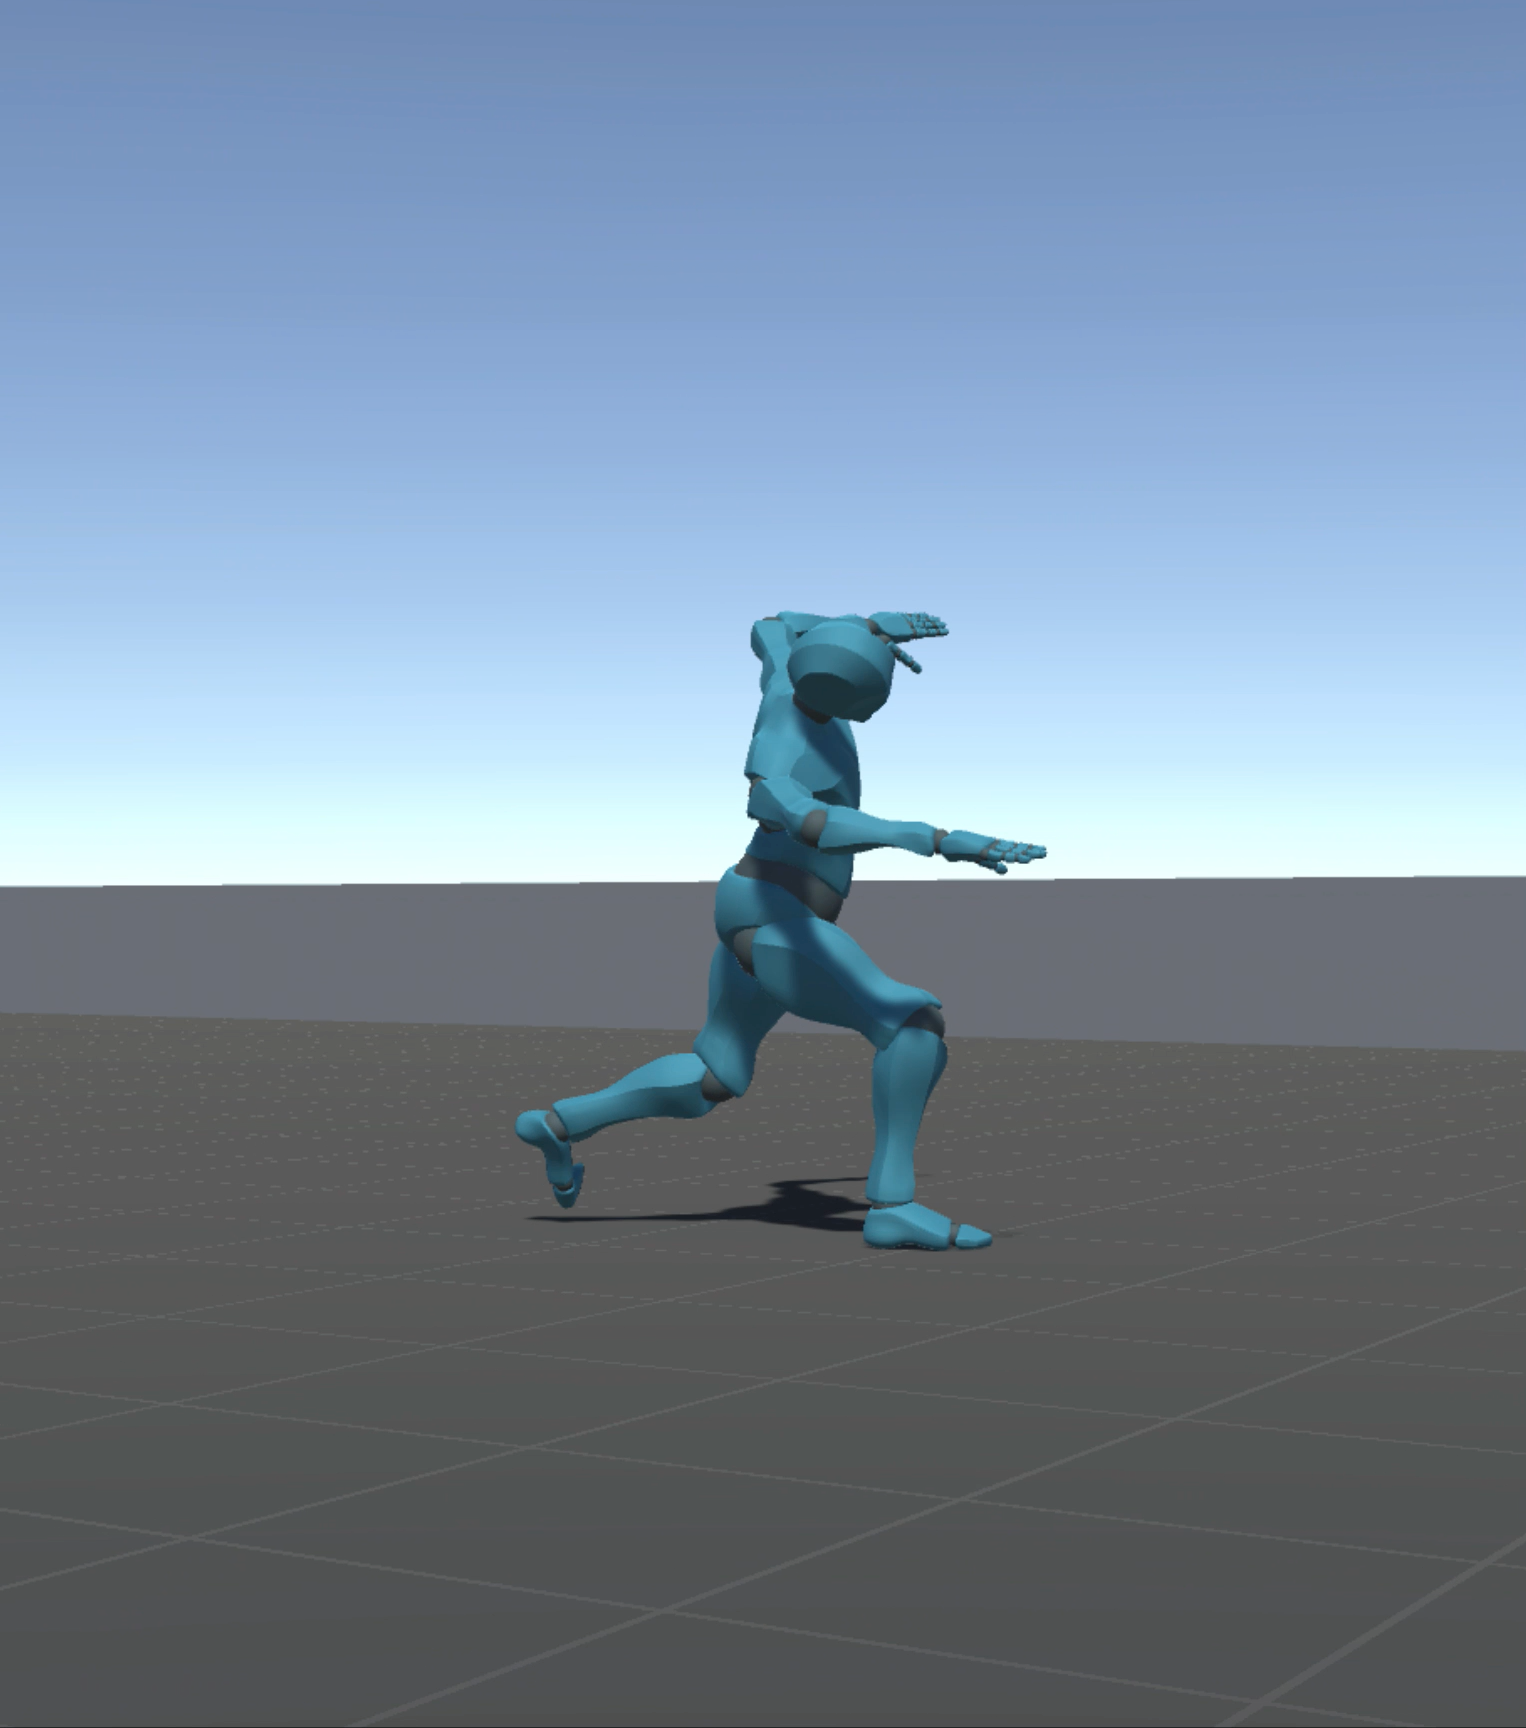
\includegraphics[width=0.2\textwidth]{img/charakter_mixamo_galoppieren2} & 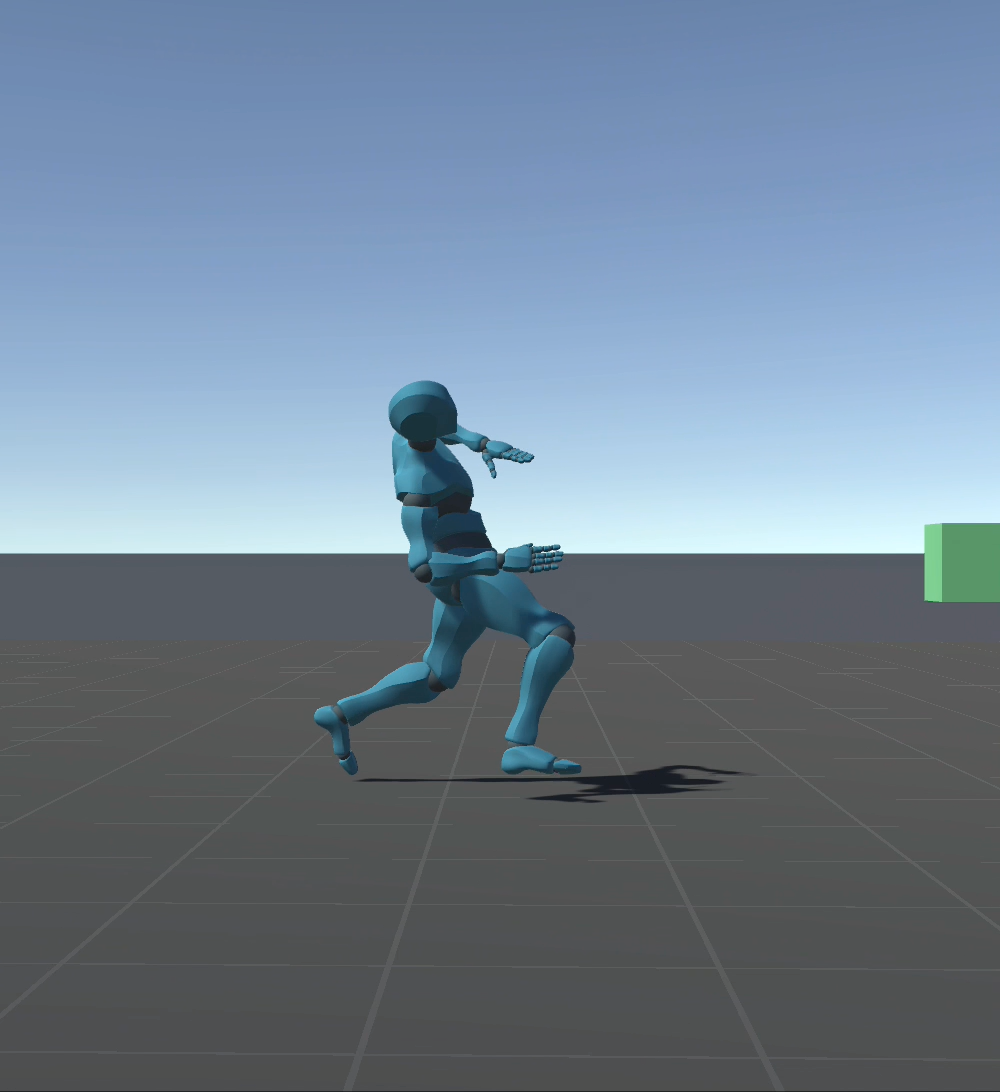
\includegraphics[width=0.2\textwidth]{img/charakter_mixamo_galoppieren3} & 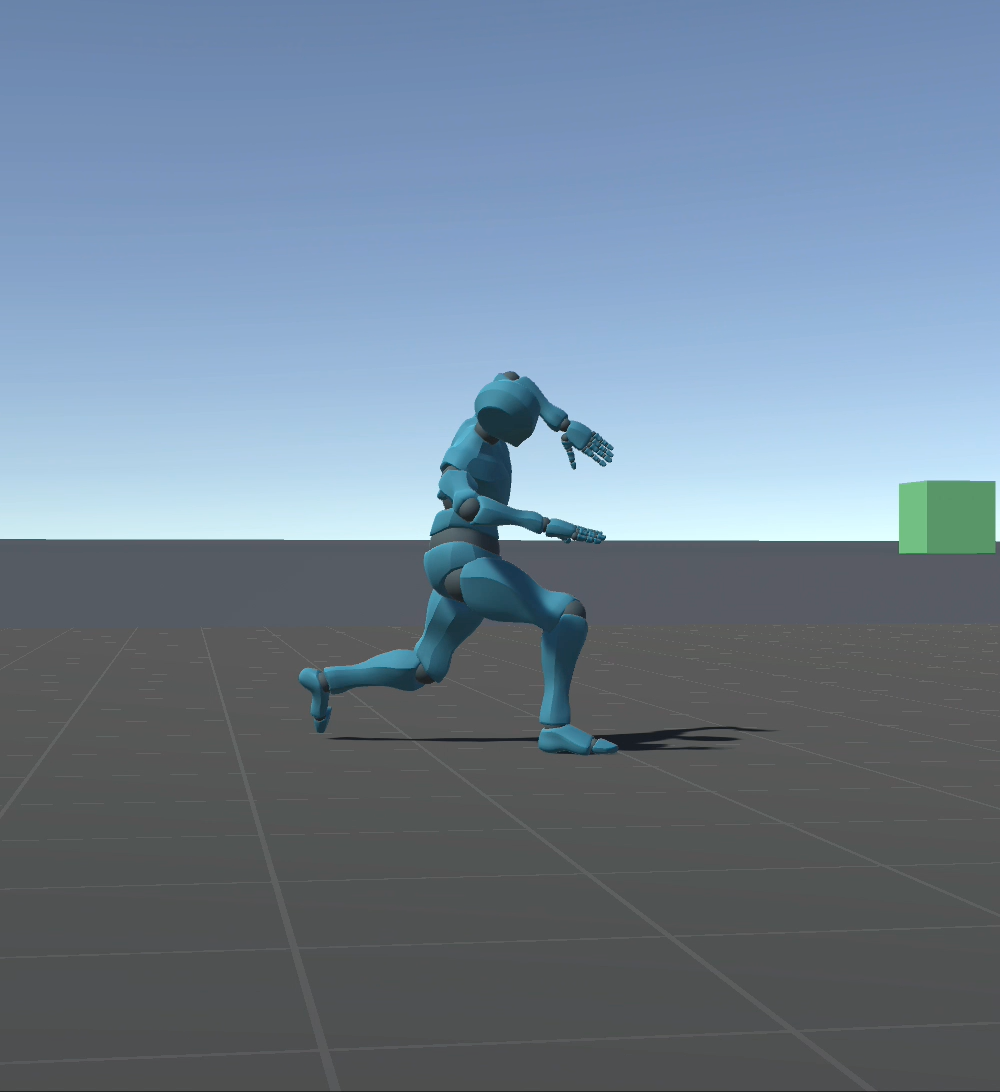
\includegraphics[width=0.2\textwidth]{img/charakter_mixamo_galoppieren4} \\
  \end{tabular}
  \caption{Mixamo Versuch 10 Gangbild}
  \label{fig:mixamo_versuch10_gangbild}
\end{figure}